% ********** Chapter 6 **********
\chapter{Skip List}
\label{sec:Hoofdstuk 6}

<<<<<<< HEAD
Intro
Naast bomen zijn er ook andere manieren om zoekalgoritmen te implementeren. In dit hoofdsuk zal een van deze structuren behandeld worden, namelijk de skip list. Een skip list bestaat uit een aantal lijsten waarvan elke lijst een subset van de lijst onder hem bevat. De onderste lijst bevat alles waardes van de boom. Elke lijst bevat in ieder geval de waardes -$\infty$ en $\infty$. Hierdoor zullen alle waardes in de lijst tussen deze twee waardes in zitten.
=======
\begin{figure}[h]
	\centering
		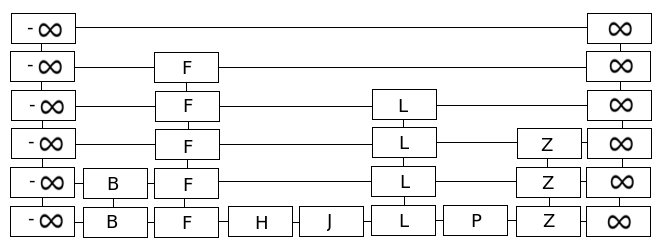
\includegraphics[width=\textwidth]{chap6/skiplist}
	\label{fig:skiplist}
\end{figure}
>>>>>>> ae6ca2bd29bdc21c848fec602c2c6eea1e9d4d0c

\section{Introductie}
Naast bomen zijn er ook andere manieren om zoekalgoritmen te implementeren. In dit hoofdsuk zal een van deze structuren behandeld worden, namelijk de skip list. Een skip list bestaat uit een aantal lijsten waarvan elke lijst een subset van de lijst onder hem bevat. De onderste lijst bevat alles waardes van de boom. Elke lijst bevat in ieder geval de waardes -\infty en \infty. Hierdoor zullen alle waardes in de lijst tussen deze twee waardes in zitten.\\
\\
\section{Zoeken}
Bij het zoeken naar een waarde $k$ in een skiplist wordt begonnen in de meest linkse waarde in de bovenste lijst, deze waarde noemen we $p$. Hierna zal gekeken worden in de waarde onder $p$, als deze niet leeg is wordt dit de nieuwe waarde van $p$. Vervolgens wordt gekeken naar de waardes aan de rechterkant van $p$. Er wordt naar rechts gezocht tot er een waarde gevonden wordt hoger dan $k$, $p$ wordt nu de waarde voor de laatst gevonde waarde. Dit wordt gedaan tot de gezochte waarde wordt gevonden. Wanneer $k$ niet in de skip list zit wordt de hoogst mogelijke waarde voor $k$ gereturned.\\
\\
\section{Toevoegen}
Bij het toevoegen van waarde $k$ wordt eerst gezocht naar $k$ op de manier zoals hierboven beschreven is. Als de gevonden waarde $p$ gelijk is aan $k$ zal direct gestopt worden, de waarde zit namelijk al in de skip list. Wanneer deze niet gelijk is zal de waarde toegevoegd worden na $p$. Hierna zal $k$ toegevoegd worden zolang een random getal tussen de 0 en 1 lager is dan 0.5.\\
\\
\section{Verwijderen}
Bij het verwijderen van een waarde $k$ zal eerst gezocht worden op deze waarde. Als de gevonden waarde $p$ niet gelijk is aan $k$ zal direct gestopt worden, $k$ zit niet in de skip list. Wanneer $k$ en $p$ wel gelijk zijn zal $p$ verwijderd worden samen met alle waardes boven $p$.\\
\\
\section{Analyse}

% ********** End of chapter **********